\listfiles
\documentclass[acmtog,review]{acmart}
%\documentclass[acmtog,anonymous,review]{acmart}
% reviewing for Class projects will be single blind.  Do not use the anonymous option.
%\setcitestyle{super,sort&compress}
\citestyle{acmauthoryear}
\usepackage{booktabs} % For formal tables

\usepackage[ruled]{algorithm2e} % For algorithms
\usepackage{lipsum}
\usepackage[english]{babel}
\usepackage{blindtext}
\usepackage{minted}
\newcommand\numberthis{\addtocounter{equation}{1}\tag{\theequation}}

% Metadata Information
%\acmJournal{CIE}
%\acmVolume{9}
%\acmNumber{4}
%\acmArticle{39}
%\acmYear{2010}
%\acmMonth{3}

%\acmBadgeL[http://ctuning.org/ae/ppopp2016.html]{ae-logo}
%\acmBadgeR[http://ctuning.org/ae/ppopp2016.html]{ae-logo}

% Copyright
\setcopyright{none}
%\setcopyright{acmcopyright}
%\setcopyright{acmlicensed}
%\setcopyright{rightsretained}
%\setcopyright{usgov}
%\setcopyright{usgovmixed}
%\setcopyright{cagov}
%\setcopyright{cagovmixed}

% DOI
\acmDOI{0000001.0000001}


% Document starts
\begin{document}
% Title portion
\title{Interactive Air-Water-Fluid Interactions Using SPH}
% \titlenote{This is a titlenote}
% \subtitle{This is a subtitle}
% \subtitlenote{Subtitle note}

% add author information here, but note that your submission should be anonymous on easychair!  
\author{William Tremblay}
\affiliation{%
  \institution{McGill University}
}
\email{william.f.tremblay@mail.mcgill.ca}

\renewcommand\shortauthors{Tremblay, W.}

\begin{abstract}
This paper presents a Rust implementation of a SPH (Smoothed Particle Hydrodynamics) model extended to model complex interactions between different fluids of different types and air. The model can simulate (im)miscibility of fluids due to polarity, temperature diffusion, effects of temperature on density, and trapped air pockets inside fluids. The implementation is multi-threaded, makes use of a cache-friendly spatial hashing approach, and dynamically generates air particles only when needed. This allows interactive simulations with up to tens of thousands of particles at fine time-steps.

\vspace{1em}
{\bf Code: \url{https://github.com/tremwil/rust_sph}}

{\bf Video: \url{https://youtu.be/Yw7QlvvZDig}}

\end{abstract}


%
% The code below should be generated by the tool at
% http://dl.acm.org/ccs.cfm
% Please copy and paste the code instead of the example below.
%
% \begin{CCSXML}
% <ccs2012>
%  <concept>
%   <concept_id>10010520.10010553.10010562</concept_id>
%   <concept_desc>Computer systems organization~Embedded systems</concept_desc>
%   <concept_significance>500</concept_significance>
%  </concept>
%  <concept>
%   <concept_id>10010520.10010575.10010755</concept_id>
%   <concept_desc>Computer systems organization~Redundancy</concept_desc>
%   <concept_significance>300</concept_significance>
%  </concept>
%  <concept>
%   <concept_id>10010520.10010553.10010554</concept_id>
%   <concept_desc>Computer systems organization~Robotics</concept_desc>
%   <concept_significance>100</concept_significance>
%  </concept>
%  <concept>
%   <concept_id>10003033.10003083.10003095</concept_id>
%   <concept_desc>Networks~Network reliability</concept_desc>
%   <concept_significance>100</concept_significance>
%  </concept>
% </ccs2012>
% \end{CCSXML}

% \ccsdesc[500]{Computer systems organization~Embedded systems}
% \ccsdesc[300]{Computer systems organization~Redundancy}
% \ccsdesc{Computer systems organization~Robotics}
% \ccsdesc[100]{Networks~Network reliability}

%
% End generated code
%

\keywords{fluid simulation, smoothed particle hydrodynamics, two dimensional, fluid-fluid interaction, air-fluid interaction, optimization, Rust}

\maketitle

\section{Introduction}
Interactions between multiple fluids, especially immiscible ones, can generate captivating emulsion patterns that can be particularly visually appealing, such as those created by lava lamps. However, reproducing such phenomena using computer simulation appears to be a rather complex endeavor, especially when one attempts to capture all particularities of such interactions. Hence we consider the use of smoothed particle models (SPH) to approximate these phenomena so that they can be simulated at interactive rates. 

\section{Related Work}
The main ideas behind this SPH implementation come from \cite{muller3} and \cite{muller5}. The former describes a simple, single-fluid SPH model which is used as a basis for the multi-fluid model developed in \cite{muller5}. Some modifications to these methods have nonetheless been made, and will be discussed in the following section.

\section{Methods}

\subsection{Base SPH Model}
The fundamental idea behind this multiple-fluid model is the single-fluid SPH model described by \cite{muller3}. Their method involves discretizing a property $\alpha$ of the fluid by encoding said property into a finite set of \textit{particles} indexed $1, \ldots, n$, and approximating its value using a \textit{smoothing kernel} $W(\vec{r},h)$:
\begin{equation}
  \label{interp}
  \alpha(\vec{x}) = \sum_{j=1}^n \alpha_j \frac{m_j}{\rho_j} W(\vec{x} - \vec{p}_j, h)
\end{equation}
where $m_j$, $\rho_j$ and $\vec{p}_j$ are the mass, density and position of particle $j$, respectively, and $h$ is the \textit{interaction}, or \textit{sampling} radius. Since the gradient, Laplacian and divergence of the above equation depends only depend on that of $W$ by linearity, one can write, say, the Navier-Stokes equations under an SPH formulation. Doing so, \cite{muller3} obtain, for particle $i$: 
\begin{align*}
  \label{smoother}
  \rho_i = \sum_{j=1}^n m_j W(\vec{p}_i - \vec{p}_j, h) \numberthis \\
  f_i^{\text{pressure}} = -\sum_{j=1}^n p_j \frac{m_j}{\rho_j} \nabla W(\vec{p}_i - \vec{p}_j, h) && \\
  f_i^{\text{viscosity}} = \mu \sum_{j=1}^n \vec{v}_j \frac{m_j}{\rho_j} \nabla^2 W(\vec{p}_i - \vec{p}_j, h)
\end{align*}
where $p_j$ is the pressure of particle $j$, which the authors compute as $k(\rho_J - \rho_0)$ for some constant $k$ and rest density of the fluid $\rho_0$, $\mu$ is the fluid's viscosity, and $\vec{v}_j$ is the velocity of particle $j$. However, one might note that the $f_i$ above are not symmetric; as such the authors replace them with the following:
\begin{align}
  f_i^{\text{pressure}} = -\sum_{j=1}^n \frac{p_i + p_j}{2} \frac{m_j}{\rho_j} \nabla W(\vec{p}_i - \vec{p}_j, h) && \\
  f_i^{\text{viscosity}} = \sum_{j=1}^n \mu \frac{\vec{v}_j - \vec{v_i}}{2} \frac{m_j}{\rho_j} \nabla^2 W(\vec{p}_i - \vec{p}_j, h)
\end{align}
These equations transfer directly to the multiple fluid case, except for (3) in which \cite{muller5} let
\begin{equation*}
  \mu = \frac{\mu_i + \mu_j}{2}
\end{equation*}
so that symmetry holds. 

The original model uses a leapfrog integration scheme, but we have found sympletic Euler to be sufficient while requiring less information to be stored inside the particle objects. 
\subsection{Collision Detection and Resolution}
For collision detection, a straightforward approach similar to that described by \cite{muller3} is used, which involves computing the axis of least separation of the particle's position with the boundary object, pushing it out, and reflecting its velocity along the axis. However, in this paper we instead compute a radius for the particle as follows: 
$$r_i = \frac{1}{2}\sqrt{\frac{m_i}{\rho_i}}$$
and resolve the circle collision instead. This does not appear to affect the visual accuracy of the simulation, but it does avoid rendering artifacts caused by particles pushed completely against the surface. 

\subsection{Interface and Surface Tensions}
\label{interface}
To simulate attraction and repulsion forces due to polarity differences, we follow \cite{muller5} and define two additional scalar fields $c^s$ and $c^i$ on the particles. $c^s$ is set 1 for all liquid particles and thus encodes liquid-air boundaries, while $c^i$ is set to $\pm 1/2$ depending on the polarity of the particle to encode boundaries between immiscible liquids. The interface and surface forces are then given by 
\begin{align}
  f_i^{\text{interface}} = -\sigma^i \nabla^2 c^i  \frac{\nabla c^i}{|\nabla c^i|}, \qquad f_i^{\text{surface}} = -\sigma^s \nabla^2 c^s  \frac{\nabla c^s}{|\nabla c^s|},
\end{align}
where the gradients and laplacians are computed by linearity according to Eq. (\ref{interp}).  

\subsection{Heat Diffusion}
The heat diffusion model is very simple and follows \cite{muller5} exactly. The heat equation being $u' = c \nabla^2 u$ for some constant $c$, applying Eq. (\ref{smoother}) we get 
$$u_i' = c \sum_{j} m_j \frac{u_j - u_i}{\rho_j} \nabla^2 W(\vec{p}_i - \vec{p}_j, h).$$
We integrate this using the Forward Euler method and then let the particle's rest density, $\rho_0$, be inversely proportional to the temperature.

\subsection{Trapped Air Generation}
The presence of air pockets, or ``bubbles'' in an agitated fluid is an important part of what make a fluid simulation look realistic. However, fully simulating all air particles around the fluid is prohibitively computationally expensive. Hence we muse the method for \cite{muller5} which boils down to the following conditions,
\begin{itemize}
  \item If $|\nabla c^p| > t_p$ (at liquid-vacuum boundary) and $\nabla c^p \cdot \vec{g} < 0$ (liquid surface is facing downwards), then spawn a particle at $x - d \nabla c^p$.
  \item If we have $|\nabla c^s| > t_s$ (not at liquid-air boundary) and $|\nabla c^p| > t_p$ (at liquid-vaccum boundary), or if $\rho < t_\rho$ for an air particle, delete it.
\end{itemize}
Here, $c^p$ is a smoothed variable which is $1$ for all particles, and $t_p, t_s, t_{\rho}$ all hand-tuned parameters. Additionally, an artificial buoyancy force proportional to $(\rho - \rho_0)\vec{g}$ is applied to the air particles to offset the pressure overestimate caused by low air particle counts, and allow it to rise to the surface. 

\subsection{Smoothing Kernels}
In the past sections the smoothing kernel $W$ has appeared in many equations. Following \cite{muller3}, we use 3 different kernels depending on what fluid property is being sampled. The paper provides these kernels for 3D; however, \cite{adithya12} gives their equivalent in two dimensions:
\begin{align*}
    W_{poly}(\vec{r}, h) &= \frac{4}{\pi h^8} (h^2 - ||\vec{r}||^2)^3, \\
    W_{spiky}(\vec{r}, h) &= \frac{10}{\pi h^5}(h - ||\vec{r}||)^3, \\
    W_{viscosity}(\vec{r}, h) &= \frac{10}{3\pi h^2}\left(-\frac{||\vec{r}||^3}{2h^3} + \frac{||\vec{r}||^2}{h^2} + \frac{h}{2||\vec{r}||} - 1\right).
\end{align*}
\cite{muller3} uses $W_{poly}$ for density, interface tension and heat diffusion, but in 2D this kernel's sign-switching Laplacian appears to be a much bigger issue and leads to heat values diverging. This may be because the ``volume'' stored in the outer ring where this sign change occurs is more significant due to the reduced dimensionality. Hence after some experimentation, this implementation uses $W_{spiky}$ for density and pressure calculations, $W_{viscosity}$ viscosity and heat diffusion, and $W_{poly6}$ for interface forces.  

\subsection{Optimizations}
To speed up the simulation, we use two ideas: spatial hashing and parallelism. The spatial hash data structure used is given below: 
\begin{minted}[fontsize=\footnotesize]{rust}
  /// Spatial hash grid cell.
#[derive(Default, Clone)]
pub struct GridCell
{
    /// Set of particles which currently lie in this grid cell.
    pub particles: HashMap<ParticleId, FluidParticle>,
    /// Boundaries, stored in the cell to accelerate collisions. 
    pub boundaries: Vec<usize>,
    /// Interacting bodies, stored here to accelerate collisions.
    pub interacting_bodies: Vec<usize>, 
}
#[derive(Clone)]
/// Spatial hash data structure, meant to accelerate range queries. 
pub struct SpatialHash {
    cells: HashMap<IVec2, GridCell>,
    particle_cells: HashMap<ParticleId, IVec2>,
    step: f32,
    inv_step: f32,
}
\end{minted}
The hash map data structure used is from \cite{Hashbrown} and is extremely performant. Since it is not node based and instead uses quadratic probing, it boasts excellent cache performance. Hence the \texttt{FluidParticle}s are stored directly inside the \texttt{GridCells} (instead of behind a pointer) to make use of this when performing neighbor queries. Indices of boundaries and other objects with collision (particle sinks and temperature sources) are stored inside grids as well to optimize collision detection. 

To multithread the simulation without sacrificing determinism, the solid \texttt{Rayon} crate from \cite{Rayon} is used. The physics update step is split into 3 parts:
\paragraph*{Density Update} Densities are updated according to Eq. (\ref{smoother}). This is done in parallel with threads splitting the work over an equal amount of particles, then performing fast neighbor queries using the spatial hash.
\paragraph*{Smoothed Property Computations} All smoothed fluid properties, such as pressure/viscosity/interface forces, color field gradients, etc., are computed at once per particle, with the work again being split over threads and making use of the spatial hash.
\paragraph*{Integration and Other Interactions} Particle positions and velocities are updated from the previously computed forces, non-fluid heat diffusion is applied, air particles are generated and stale ones are deleted. This is all done in a single thread, but is $O(n)$ and does not appear to be a bottleneck unless the number of particles is low. Care is taken to minimize the number of unnecessary memory (de)allocations as particles are dynamically created and destroyed during this step.
% \begin{itemize}
%   \item \texttt{update_densities}: Compute and update 
% \end{itemize}

\subsection*{Rendering}
The rendering and UI components of the implementation make use of the \texttt{macroquad} Rust crate \cite{Macroquad}. With the simulation being capable of many tens of thousands of particles, another challenge arises, namely drawing them at a high resolution quickly. For this an idea by \cite{parker20} was ported to \texttt{macroquad}'s OpenGL layer. The author passes a single quad to the GPU and uses a fragment shader to draw up to millions of circles with pixel-precision by doing a single instanced draw call. This made the particle rendering multiple orders of magnitude faster than a naive loop over \texttt{macroquad}'s \texttt{draw\_circle} function. 

\section{Results}
For performance metrics, note the following was tested on a PC with 16GB of 2400MHz DDR4 RAM, an Intel i5 12600K CPU @ 4.1GHz and an NVidia RTX 3070 graphics card. 
\subsection{Stability}
One of the main issues with a SPH model that isn't divergence free is that to make liquids appear non-compressible, they must be assigned a very high stiffness $k$. This leads to large pressure forces that require careful either aggressive damping via high viscosities or taking small timesteps. In our tests, we have found that a viscosity of 1 and stiffness of 50 produced visually appealing results, even though water's real viscosity is two orders of magnitude lower. For most examples, we use timesteps of $0.0005$ seconds, but the simulator can usually ensure stability up to $0.002$ seconds or more depending on particle size and count. 

\subsection{Multiple-Fluid Interactions}
Blobs of water (1000$kg/m^2$) and oil (900$kg/m^2$) were dropped into ethanol ($789kg/m^2$). Both water and ethanol were modeled as polar, while oil was made non-polar, leading to emulsion at the boundary. The fluids unmixed themselves due to density differences (Fig. \ref{interface}). 
\begin{figure}[h]
  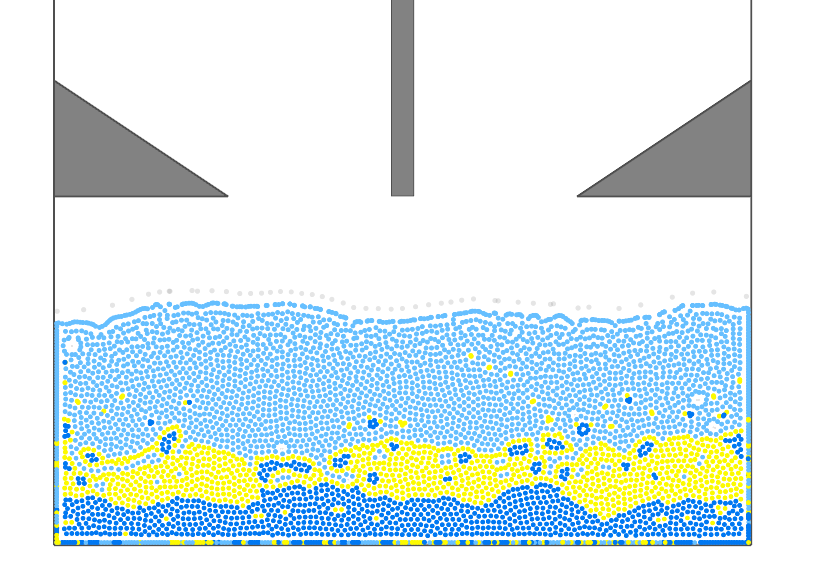
\includegraphics[width=0.4\textwidth]{interface.PNG}
  \caption{Oil, water and EtOH are mixed together.}
  \label{interface}
\end{figure}

\subsection{Trapped Air}
In this test, an emitter generates water particles at a rate of 3000/s, while a sink under the circle destroys them. The particles collide with the circle and form droplets that fall in the pool of fluid below, creating many air bubbles (white) (Fig \ref{bubbles}).
\begin{figure}[h]
  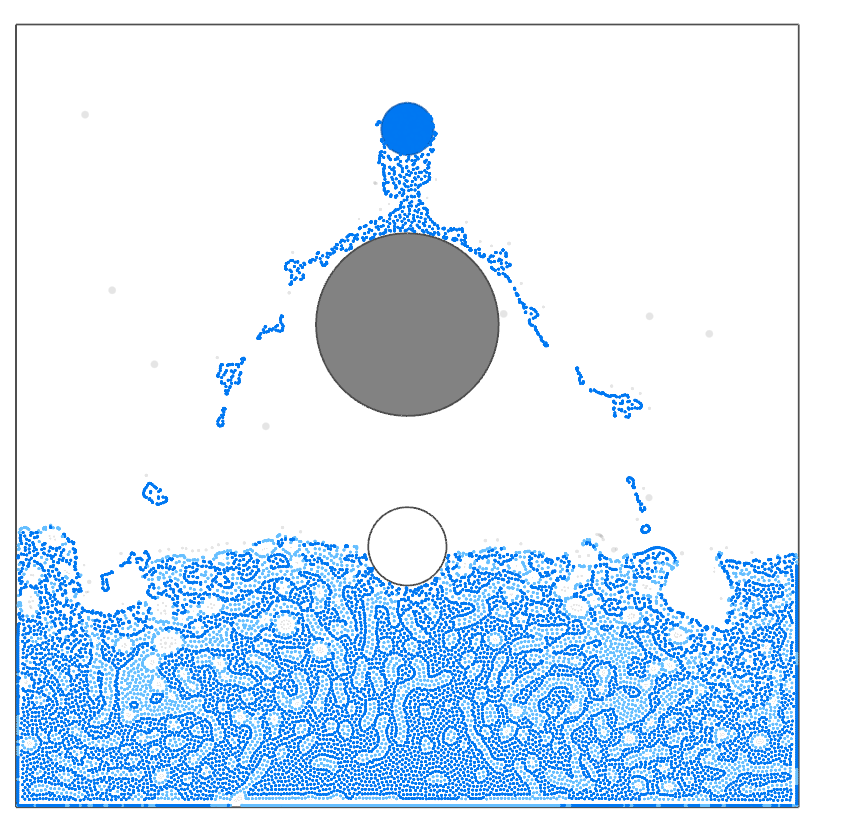
\includegraphics[width=0.4\textwidth]{bubbles.PNG}
  \caption{Fluid droplets fall and create bubbling.}
  \label{bubbles}
\end{figure}

\subsection{Heat Diffusion}
Heat and cold sources (set to 500K and 100K respectively) were placed at each end of the fluid to create a temperature gradient. The fluid density changed as its temperature did, leading to buoyancy forces, that initiated a current in the fluid (Fig. \ref{diffuse}). This test used 3306 particles and ran at 50\% real time, with a timestep of 1/1440s. 
\begin{figure}[h]
  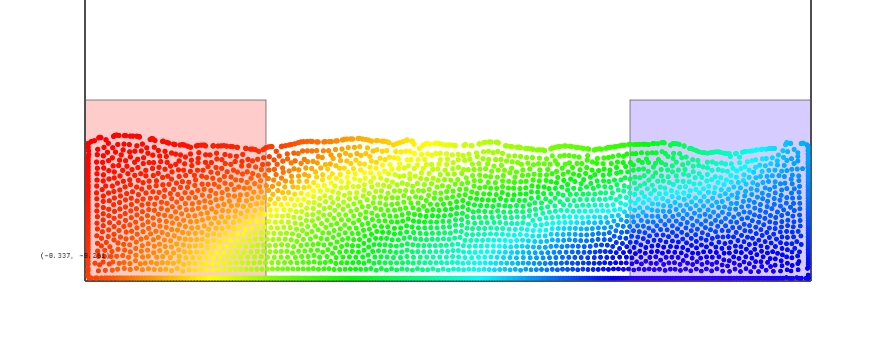
\includegraphics[width=0.4\textwidth]{diffusion.PNG}
  \caption{A temperature gradient induces a current inside the fluid.}
  \label{diffuse}
\end{figure}

\subsection{Performance}
Three test scenes have been created to assess the model's performance. In the first, a 4585-particle dam-break scenario is played at 1/3 real-time speed at 60 frames per second, using a time step of $1/180$ with $7$ substeps. Hence each physics update took $1/420 \approx 2.3$ milliseconds. The second involves two 20,000 1mm fluid blocks, one of water and one of oil, colliding into one another at a relative speed of 2 $m/s$ (Fig. \ref{stress1}). Oil density was set to half that of water, which is set to $1000kg/m^2$.  Trapped air bubbles can also be seen.
\begin{figure}[h]
    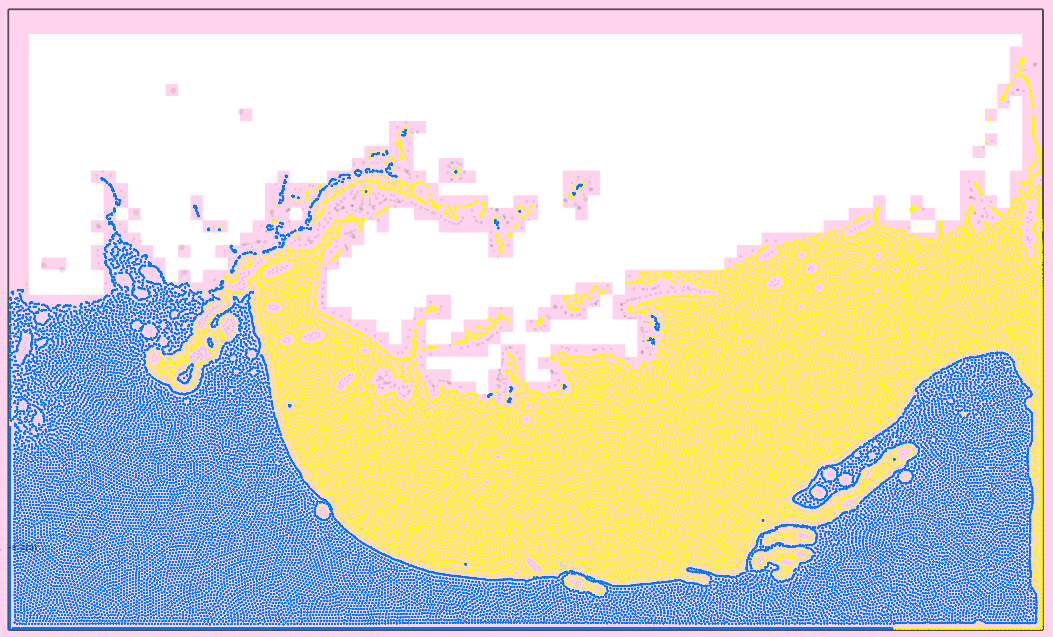
\includegraphics[width=0.4\textwidth]{stress_test_1.PNG}
    \caption{Result of two 20K cubes of fluid slamming into one another.}
    \label{stress1}
\end{figure}
The last scene is a 100 thousand particle stress test, where a block of fluid moving to the right impacts a sphere and then a ball (Fig. \ref{stress2}). Timestep was set to 0.0005 seconds, and the simulation ran at 10 frames per second, or about 100ms per physics update. 
\begin{figure}[h]
  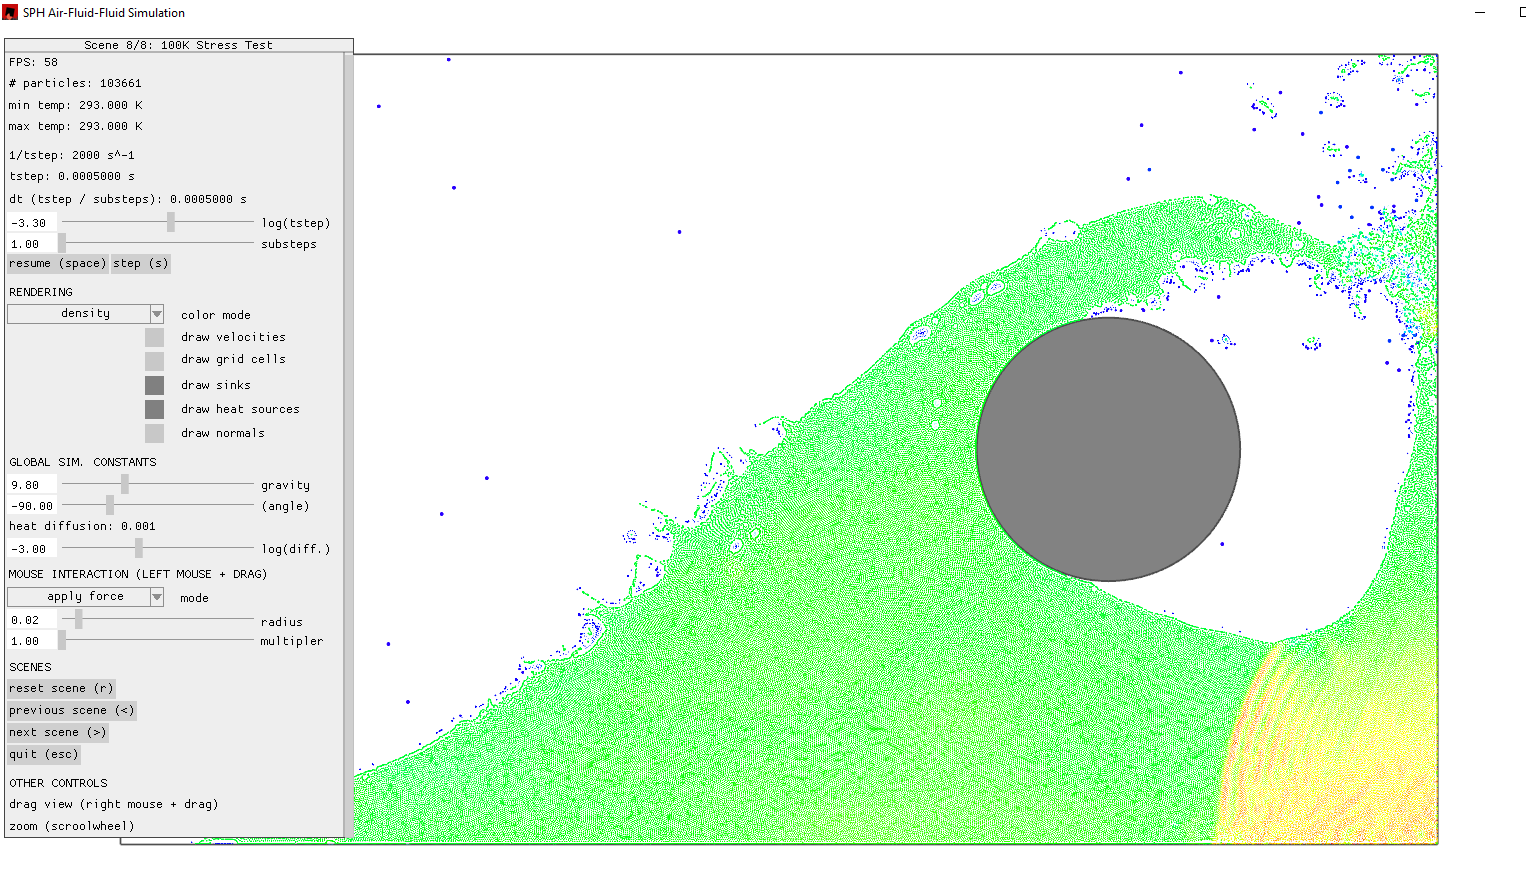
\includegraphics[width=0.4\textwidth]{stress_test_2.PNG}
  \caption{100K particle cube colliding into a sphere. Particles are \\ 
  colored according to their density. Generated air particles can be seen . }
  \label{stress2}
\end{figure}

\section{Conclusions}
A high-performance Rust implementation of a multi-fluid SPH model capable of handling many different types of fluid interactions was presented. The model also accounts for trapped air particles, and is able to simulate density changes caused by heat transfer.

% Bibliography
\bibliographystyle{ACM-Reference-Format}
\bibliography{projectBibliography}


\end{document}
